\section{Was sind Quanten?}
\begin{frame}
	\frametitle{Ursprung des Begriffs}
  \begin{columns}
	\begin{column}{0.48\linewidth}
		\img{0.75\linewidth}{Kommunikation/Democritus}{quantum:democritus}{Demokrit (460–371 v. Chr.)}{Demokrit (460–370 v. Chr.)}
		% Quelle: https://commons.wikimedia.org/wiki/File:Democritus2.jpg#filelinks
	\end{column}
	\begin{column}{0.48\linewidth}
		\justifying
		-- Quant = lat. \enquote{quantum} \textrightarrow{ }\enquote{wie groß} / \enquote{wie viel}\\
		-- Bedeutet messbares, quantifizierbares\\
		-- Demokrit: Materie nicht unendlich teilbar \textrightarrow{ }Atome
	\end{column}
\end{columns}
\end{frame}

\begin{frame}
	\frametitle{Der Photoeffekt}
	\begin{columns}
		\begin{column}{0.48\linewidth}
			\justifying
			Thomas Young:\\
			Doppelspaltversuch (1801 bis 1803) \textrightarrow
			{ }Licht = Welle mit typischen Überlagerungsmuster (Interferenz)
		\end{column}
		\begin{column}{0.48\linewidth}
			\img{1.15\linewidth}{Kommunikation/Double-slit-exp}{quantum:double_split}{Doppelspalt}{Doppelspalt}
			% Quelle: https://commons.wikimedia.org/wiki/File:Democritus2.jpg#filelinks
		\end{column}
	\end{columns}
\end{frame}

\begin{frame}
	\frametitle{Natur des Lichts}
	\begin{columns}
		\begin{column}{0.48\linewidth}
%			\justifying
			-- Licht l{\"o}st Elektronen aus Metalloberflächen\\
			-- Stromfluss abh{\"a}ngig von der Farbe (Frequenz), nicht Helligkeit (Erwartung)\\ 
			-- Albert Einstein (Idee von Max Planck):\\
			\hspace{0.8em} -- Licht tritt in Energiepaketen\\
			\hspace{1.5em} (Photonen) \textbf{\textrightarrow}\\
			\hspace{1.5em} Teilcheneigenschaft\\
			\textbf{\textrightarrow{ }Wellen-Teilchen Dualismus}
		\end{column}
		\begin{column}{0.48\linewidth}
			\img{0.85\linewidth}{Kommunikation/Photoelectric_effect}{quantum:wave_dual}{Photoelektrischer Effekt}{Photoelektrischer Effekt}
			% Quelle: https://commons.wikimedia.org/wiki/File:Democritus2.jpg#filelinks
		\end{column}
	\end{columns}
\end{frame}

\begin{frame}
	\frametitle{Beispiele für Quantenobjekte}
	\begin{columns}
		\begin{column}{0.33\linewidth}
			\centering
			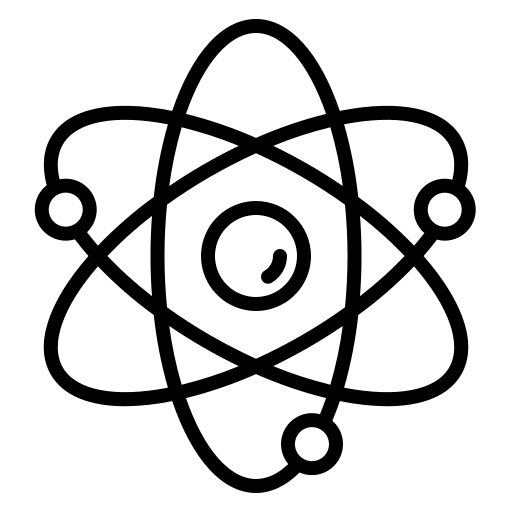
\includegraphics[scale=0.15]{figures/Kommunikation/atom.png}\\
			Elektronen \& Quarks
		\end{column}
		\begin{column}{0.33\linewidth}
			\centering
			
\includegraphics[scale=0.12]{figures/Kommunikation/sonne.png}\\
			Photonen \& Gluonen
		\end{column}
		\begin{column}{0.33\linewidth}
			\vspace*{0.75em}\\
			\centering
			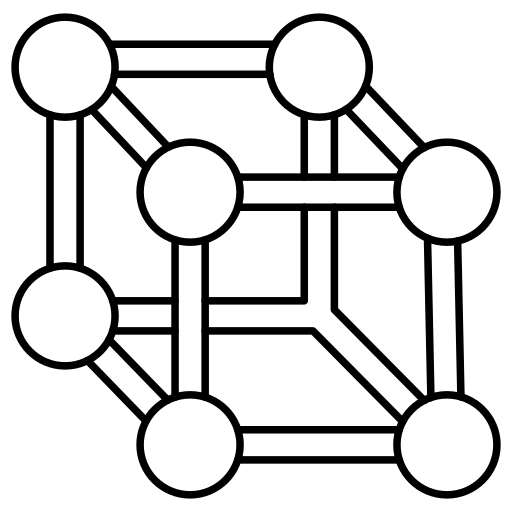
\includegraphics[scale=1.2]{figures/Kommunikation/molekul.png}\\
			Gitterschwingungen in Kristallen
		\end{column}
	\end{columns}
\end{frame}